\section{Linearisieren}
\subsection{Least Square}
Findet eine Gerade welche die Varianz, Quadratischer Abstand von Gerade, minimiert. 
\begin{center}
	\begin{minipage}{0.20\textwidth}
		\begin{center}
			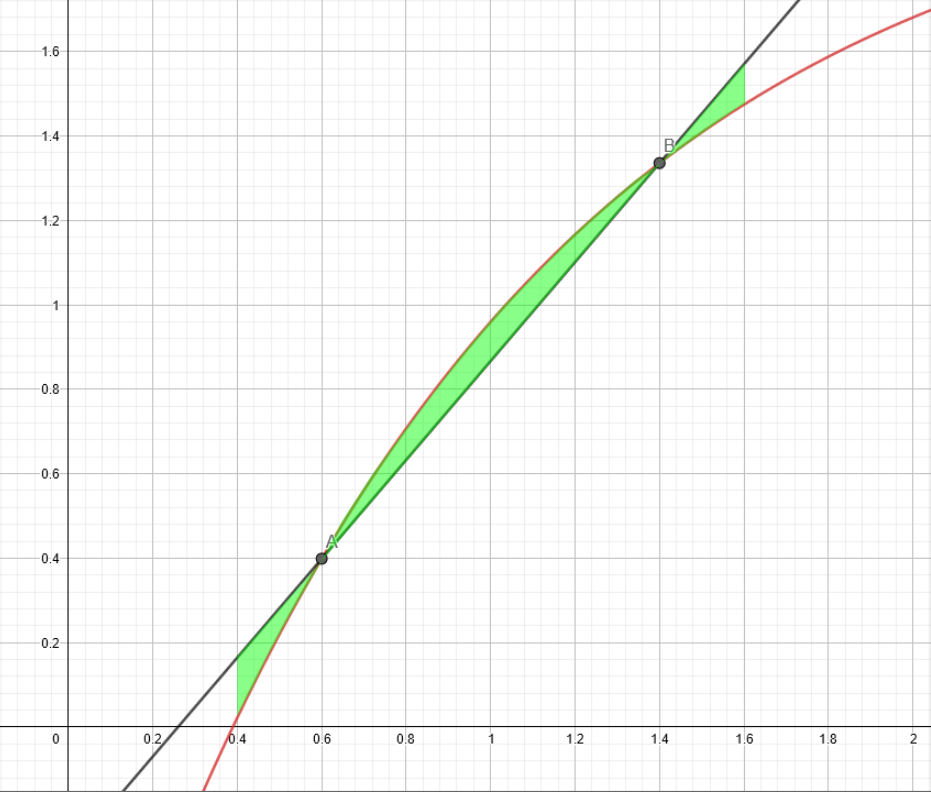
\includegraphics[width=\linewidth,keepaspectratio=true]{Images/leastsquare}\\
		\end{center}
	\end{minipage}%%% to prevent a space
	\begin{minipage}{0.3\textwidth}
		\[\textcolor{red}{\vec{x}} = (A^TA)^{-1}A^T\vec{b}\]
	\end{minipage}
\end{center}

\noindent
Beispiel für \textbf{streng Lineares System} ($b=0$): $y_i = \textcolor{red}{a}x_i$.
\[
\underbrace{\begin{pmatrix}
		x_1 \\
		x_2 \\
		\vdots \\
		x_n
\end{pmatrix}}_{\scriptsize{A}}
\cdot
\underbrace{\begin{pmatrix}
		\textcolor{red}{a}
\end{pmatrix}}_{\scriptsize{\textcolor{red}{\vec{x}}}}
=
\underbrace{\begin{pmatrix}
		y_1 \\
		y_2 \\
		\vdots \\
		y_n
\end{pmatrix}}_{\scriptsize{\vec{b}}}
\]

\noindent
Beispiel für \textbf{nicht Lineares System} ($b\neq0$): $y_i = \textcolor{red}{a}x_i + \textcolor{red}{b}$.
\[
\underbrace{\begin{pmatrix}
		x_1 & 1 \\
		x_2 & 1 \\
		\vdots & \vdots \\
		x_n & 1
\end{pmatrix}}_{\scriptsize{A}}
\cdot
\underbrace{\begin{pmatrix}
		\textcolor{red}{a} \\
		\textcolor{red}{b}
\end{pmatrix}}_{\scriptsize{\textcolor{red}{\vec{x}}}}
=
\underbrace{\begin{pmatrix}
		y_1 \\
		y_2 \\
		\vdots \\
		y_n
\end{pmatrix}}_{\scriptsize{\vec{b}}}
\]
